\section{Busauslastung messen}
Um zu beurteilen, ob Bluetooth Low Energy (BLE) eine geeignete Lösung für die Übertragung von Telegrammen vom Sniffer zum Endgerät darstellt, wurde die Busauslastung mit einem Picoscope aufgezeichnet und mittels Matlab ausgewertet. Ziel war es abzuschätzen, ob die effektiven Nutzdaten über BLE übertragen werden können. Gleichzeitig sollen erste Erfahrungen im Bereich der Signalauswertung gemacht werden, welche für die Implementierung im FPGA genutzt werden können.

Für die Analyse wurden zwei Messungen durchgeführt: Eine unter Normallast und eine unter Volllast. Die Volllast wurde simuliert, indem der Depot-Diagnosespeicher (DDS) auf dem Fahrzeugdisplay abgerufen wurde. Dies führte dazu, dass der Speicher die entsprechenden Daten über den Bus an das Display sendete, was kurzfristig zu einer höheren Auslastung führte.

Die Messungen wurden mit einem Picoscope 2207B durchgeführt, während die anschliessende Auswertung mit Matlab realisiert wurde.

\subsection{Messaufbau}

Der Messaufbau ist in Abbildung \ref{fig:MessaufbauBusauslastungMessen} dargestellt. Um die Busauslastung zu messen, wurde die MVB-Leitung, die normalerweise von Gerät zu Gerät durchgeschleift ist, an einer geeigneten Stelle unterbrochen und ein Leitungsaufteiler eingefügt. Dies ermöglichte den direkten Zugriff auf die differentiellen Leitungen des Busses mit dem Picoscope. Der MVB-Loop wurde dabei wieder geschlossen, sodass keine Geräte vom Bus abgetrennt wurden. Die gemessenen Daten wurden über eine USB-Schnittstelle an einen Laptop übertragen und dort mit der Pico-Software aufgezeichnet.

\begin{figure}[H]
    \centering
    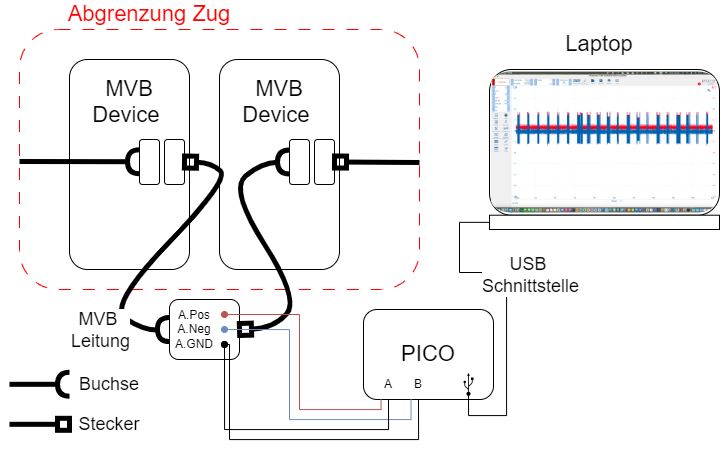
\includegraphics[width=0.8\linewidth]{Figures/Chap3/Busauslastung/Messaufbau_PICO_IC2000.png}
    \caption{Messaufbau Busauslastung messen}
    \label{fig:MessaufbauBusauslastungMessen}
\end{figure}

Die erfassten Daten wurden anschliessend in das Matlab-Dateiformat (.mat) exportiert. Die Struktur der Matlab-Datei ist in Abbildung \ref{fig:MatlabFileStruktur} dargestellt. Die Variablen \textit{A} und \textit{B} entsprechen den Messpunkten des Picoscope, während \textit{Tinterval} die Zeit zwischen zwei Messpunkten angibt. 

\begin{figure}[H]
    \centering
    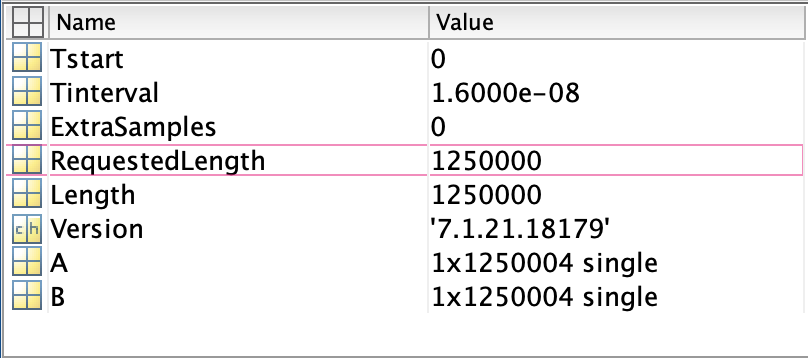
\includegraphics[width=0.5\linewidth]{Figures/Chap3/Busauslastung/Matlab_file_struktur.png}
    \caption{Matlab File Struktur}
    \label{fig:MatlabFileStruktur}
\end{figure}

Der Messaufbau blieb für die Messungen unter Normallast und Volllast identisch. Um die Volllast zu simulieren, wurde der Befehl zur Anzeige der DDS auf dem Fahrzeugdisplay ausgelöst, bevor die Messung gestartet wurde. Der Zeitraum zwischen der Eingabe des Befehls und der Darstellung der Daten auf dem Display beträgt etwa 5 Sekunden.

Das Picoscope wurde für die Messung mit einer Abtastrate von 62,5 MS/s konfiguriert, was einem Abtastintervall von 16 ns entspricht. Diese maximale Abtastrate wurde gewählt, um selbst kleinste Signaländerungen erfassen zu können. 

\subsection{Matlab Auswertung}
Die Auswertung der Analogwerte wurde mit Matlab realisiert. Ziel war es, herauszufinden, wie gross die Busauslastung in Bit/s ist. Für die Übertragung mit Bluetooth waren alle Daten ausser die Start-Delimiter (siehe Kapitel \ref{sub:StartDelimiter}) von Interesse. Die Auswertung mit Matlab diente ebenfalls als Grundlage für weitere Überlegungen, insbesondere für die spätere Implementierung im FPGA (siehe Kapitel \ref{Manchester Decodierung}). Die Auswertung ist in folgende Schritte unterteilt:
\begin{enumerate}
    \item Delimiter Erkennung
    \item Bestimmung Anzahl Bit
    \item Differenz bilden
\end{enumerate}


\subsubsection{Delimiter erkennen}
%\textcolor{red}{Anzahl delimiter erkennen. Charakteristik erkannt -> letzte werte Idle, dann Nulldurchgang, aber nur wenn einer der nächsten 20 Werte über null ist, sonst wurde peak am schluss auch gezählt. }
Um die Start-Delimiter zu erkennen, wurde die Charakteristik eines Delimiters gemäss Kapitel \ref{sub:StartDelimiter} untersucht. In Abbildung \ref{fig:AusschnittMvbOhneDds} wurde der Zeitbereich vergrössert. Dadurch lässt sich ein Telegramm (gemäss Kapitel \ref{sub:MasterSlavePrinzip}) besser sehen.

\begin{figure}[H]
    \centering
    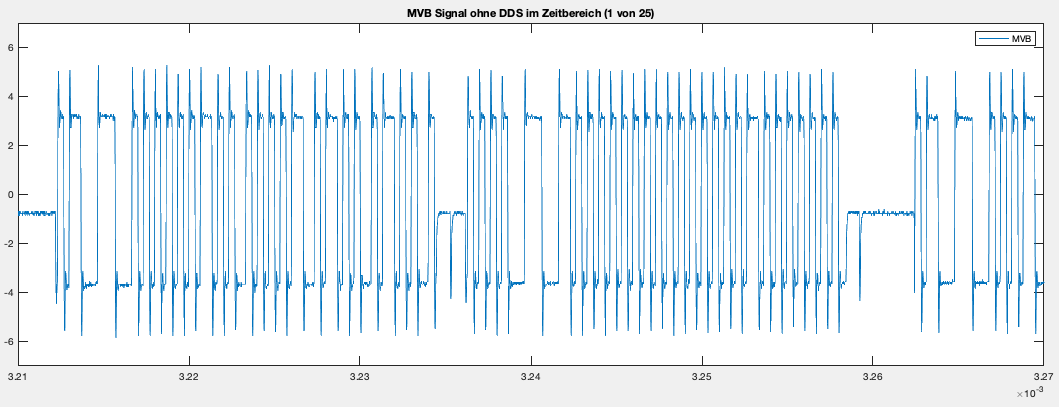
\includegraphics[width=0.8\linewidth]{Figures/Chap3/Busauslastung/Ausschnitt_MVB_ohne_Delimiter.png}
    \caption{Ausschnitt MVB Signal ohne DDS}
    \label{fig:AusschnittMvbOhneDds}
\end{figure}

Zu sehen ist, ein vollständiges Master-Frame, das darauffolgende Slave-Frame und der Anfang des nächsten Master-Frames. Das Idle Signal verbindet die Frames. Der Start-Delimiter fängt bei der ersten negativen Flanke an. Gemäss Norm muss das Slave-Frame in einem Zeitraum zwischen 2 - 6 $\mu$s folgen. \cite{MVB_Frame_space} Somit kann die Charakteristik des Start-Delimiters wie folgt zusammengefasst werden: Ist das Idle Signal für mindestens 2 μs anstehend, beginnt der Start-Delimiter bei der ersten negativen Flanke.

Diese Definition konnte so nicht umgesetzt werden, da dies zu mehreren Fehlererkennungen geführt hat, da die Periode zwischen Master- und Slave-Frame teilweise unter 2 $\mu$ s war und weil ein negativer Puls am Ende des Master- oder Slave-Frames die Bedingung der Idle-Zeit verletzte. Stattdessen wurde ein Zeitbereich von 0.5 Bitdauer gewählt und die zusätzliche Bedingung eingeführt, dass nach Erkennung einer negativen Flanke in der nächsten 0.5 Bitdauer mindestens ein Wert über 0V sein muss. Daraus gab sich der Algorithmus zur Erkennung der Start-Delimiter und die erkannten Punkte werden in Abbildung \ref{fig:enter-label} gezeigt.

\begin{figure}[H]
    \centering
    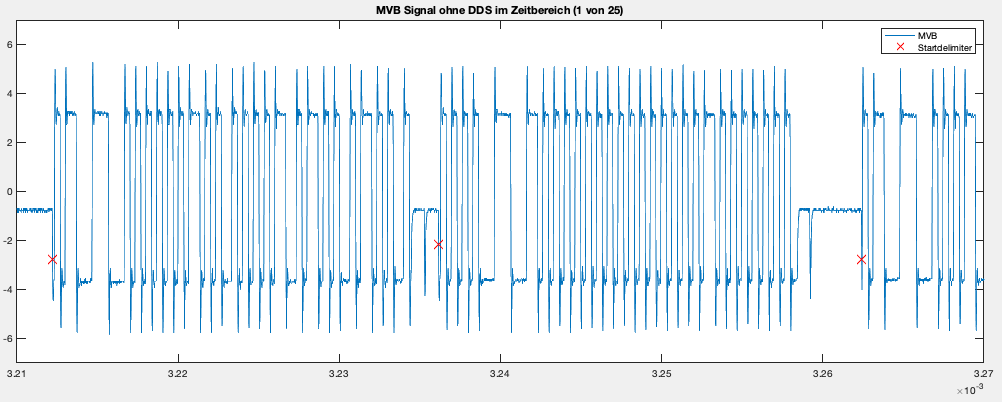
\includegraphics[width=0.8\linewidth]{Figures/Chap3/Busauslastung/Ausschnitt_MVB_mit_Delimiter.png}
    \caption{Ausschnitt der MVB Messung unter Normallast mit
Start-Delimiter Erkennung (rote X)}
    \label{fig:enter-label}
\end{figure}


\subsubsection{Anzahl Bit}
\label{subsub:Nulldurchgänge}
%\textcolor{red}{Anzahl bit mit Start-Delimiter erkennen. Als erstes alle werte zwischen 0 und -1V gelöscht, weil Idle. Dann wurde eine Flanke detektiert. Wenn eine Flanke detektier um 30 Werte vorwärts springen (damit zweite Flange nicht nochmals erkennt wird (manchester encodiertes Signal)}
In diesem Schritt wurde mit Matlab die Anzahl Bit aus der Messung ausgewertet. Gemäss Kapitel \ref{sub:BitEncoding} gibt es für den Wert "'0"' und "'1"' jeweils einen Flankenwechsel in der Hälfte der Bitdauern (BT, gemäss Kapitel \ref{sub:GeschwindigkeitDatenbus}: 1 BT = 666 ns). Dies kann verwendet werden, um die Anzahl Bit herauszufinden. Anhand Abbildung \ref{fig:Suchalgo_Bits} kann der gewählte Suchalgorithmus erklärt werden.

\begin{figure}[H]
    \centering
    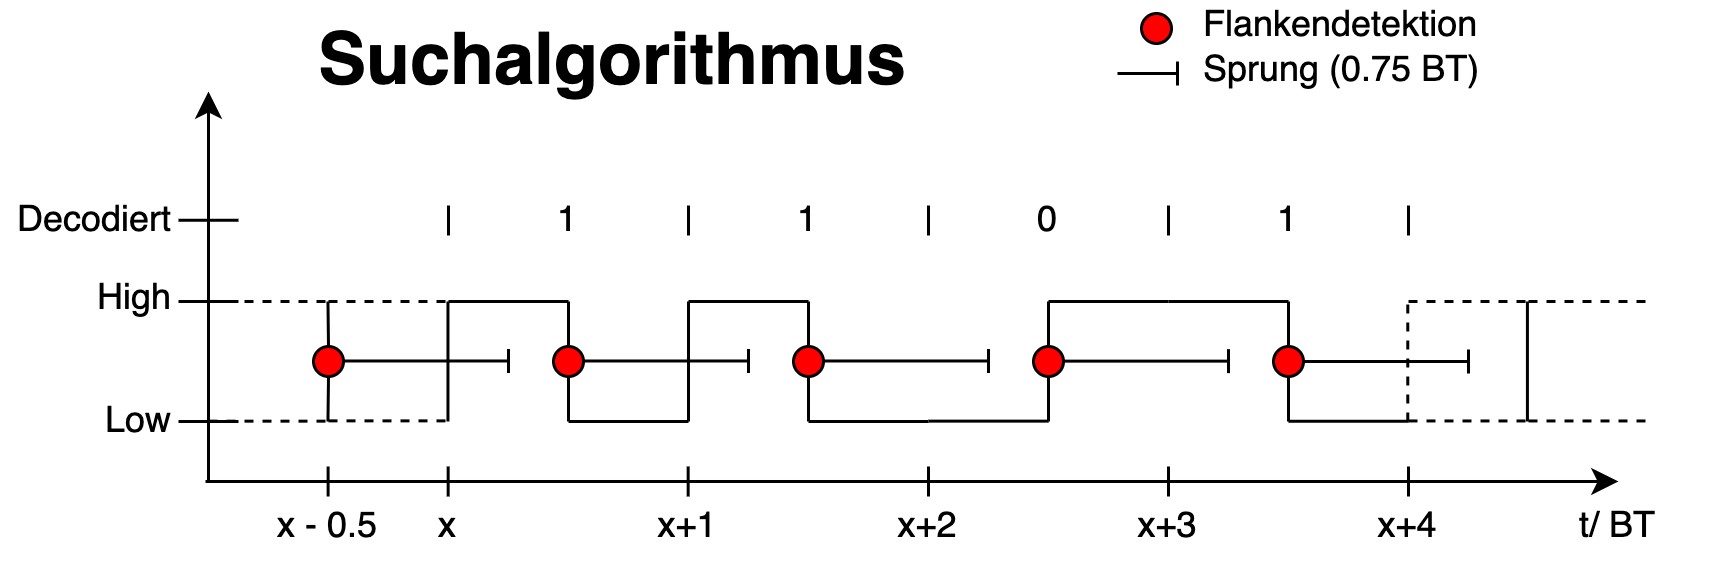
\includegraphics[width=0.9\linewidth]{Figures/Chap3/Busauslastung/Suchalgorithmus_Bits.png}
    \caption{Suchalgorithmus der Bit in einem Manchester encodierten Signal}
    \label{fig:Suchalgo_Bits}
\end{figure}

X steht für eine zufällige Zeit innerhalb einer Transaktion am Anfang eines Manchester Bit. Auf der Abszisse ist die Zeit in Bitdauer aufgetragen. Auf der Ordinate ist ein Beispielsignal und die Decodierung des Signals aufgezeigt. Da in der Mitte der Bitdauer eine Flanke zu erwarten ist, wird auch eine halbe Bitdauer vor X eine Flanke erwartet. Dies bildet den Einstieg. Wird eine Flanke detektiert, wird um eine Bitdauer von 0.75 positiv in der Zeit gesprungen. Der Sprungpfeil zeigt mit seinem flachen Ende, ab wo die nächste Flanke gesucht wird. Der Sprung erfolgt, weil Flankendetektionen wie bei \textit{x+1} in Abbildung\ref{fig:Suchalgo_Bits}, nicht berücksichtigt werden, da diese die Auswertung verfälschen.

Gemäss Anhang \ref{app:Flankenerkennung Bits} sind die Anzahl der Flanken, welche in einem Master Start-Delimiter und einem Slave Start-Delimiter gezählt werden sieben.

Für die Auswertung am MVB-Signal wurde in einem ersten Schritt das Idle-Signal, also alle Messpunkte zwischen -0.5 V und -1 V aus dem Signal entfernt. Daraus folgt ein Signal,  welches Startbit, Start-Delimiter, Master-Frame sowie Slave-Frame-Daten enthält. In Abbildung \ref{fig:ReineDaten} ist ein Vergleich zwischen beiden Signalen zu sehen: oben mit Idle-Signal, unten ohne Idle-Signal. Die Idle-Zeit macht somit 75 \% aus. Die Periodendauer des Busses gemäss Kapitel \ref{sub:PeriodeAufDemBus} ist 1 ms.

\begin{figure}[H]
    \centering
    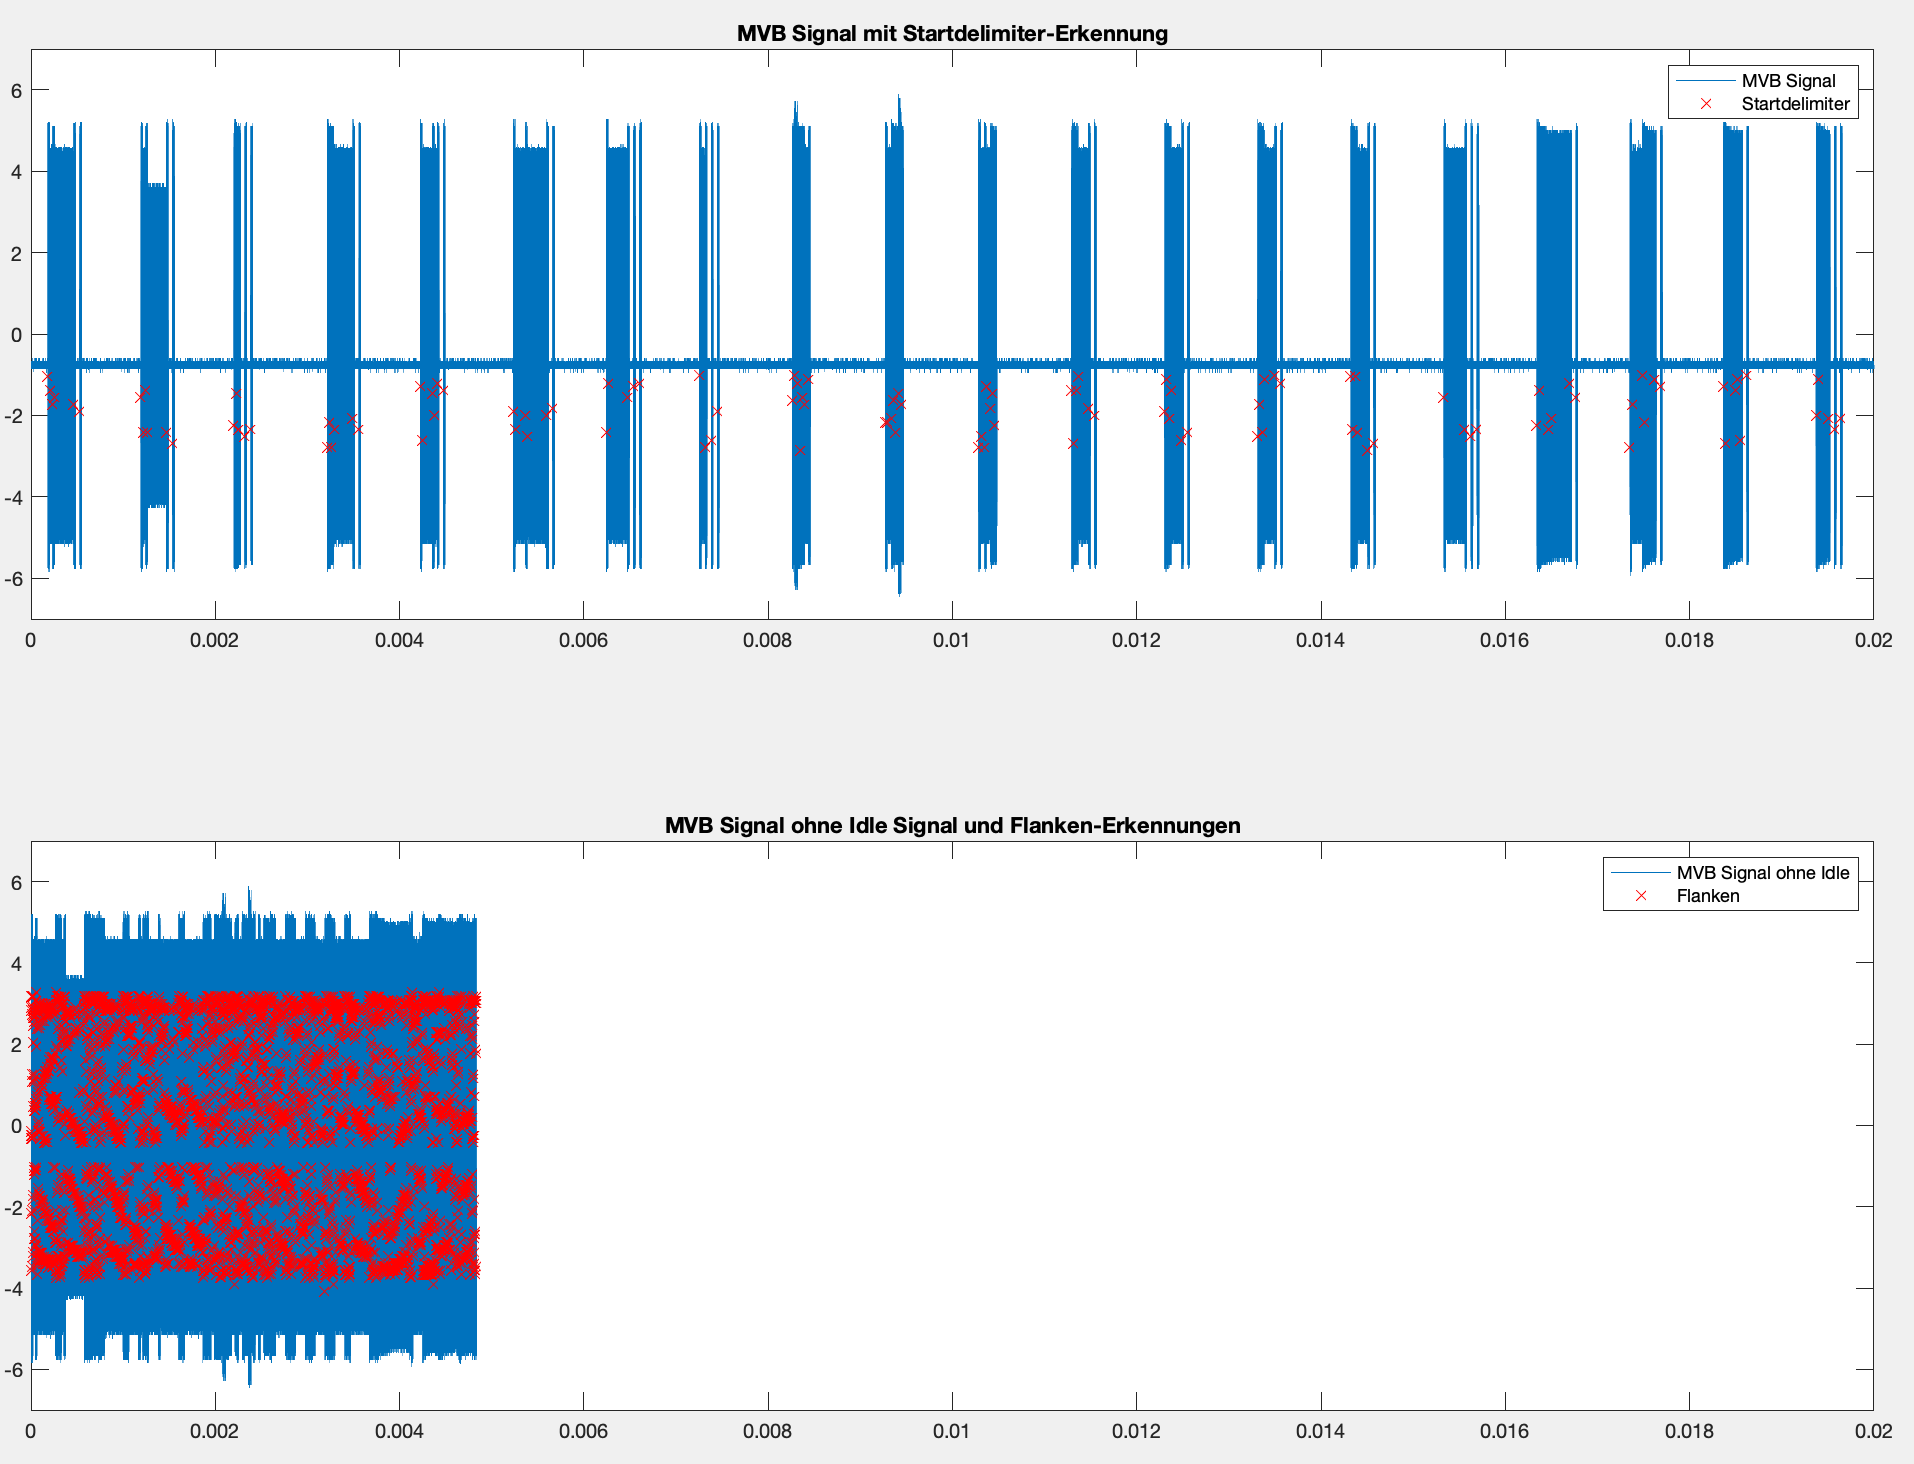
\includegraphics[width=0.75\linewidth]{Figures/Chap3/Busauslastung/Vergleich_MVB_mit_ohne_Idle.png}
    \caption{Vergleich MVB Signal mit und ohne Idle-Signal (oben und unten) über einen Zeitraum von 20 ms}
    \label{fig:ReineDaten}
\end{figure}

Der Suchalgorithmus wurde auf die Daten angewendet und die Anzahl Bit gezählt. Die Anzahl Bit sind die roten X im Plot unten. In diesem Beispiel sind es 7033 Bit, die erkannt wurden. 

\subsubsection{Auswertung effektive Nutzdaten}
%\textcolor{red}{Effektive = Anzahl Nuldurchgänge - (Delimiert * 9); Tablle effiktive Nutzwerte mit und ohne DDS.}
Anschliessend wird ausgewertet, wie viele Bit an effektivem Payload innerhalb einer Zeitdauer von 20 ms geschickt werden. Anhand Formel \ref{equ:effektivBPS} kann dies  für jede der 25 Messungen unter Normallast und unter Volllast berechnet werden.

\begin{equation}
    eff\_bps = (NumBit - (NumDelimiter * 7)) / 0.02
    \label{equ:effektivBPS}
\end{equation}


 Die Tabelle \ref{tab:Busauslastung} zeigt die Auswertung  der Busauslastung. Die Spalten 1 und 3 enthalten die minimalen sowie maximalen Werte der je 25 Messungen. Die Spalte \textit{mean} wurde mit dem Matlabbefehl \textit{mean()} berechnet und gibt den Mittelwert über die je 25 Messungen aus. 

\begin{table}[H]
    \centering
    \begin{tabular}{r|c|c|c}
        & min in Bit/s & mean in Bit/s & max in Bit/s\\ 
        \hline
        Normallast & 2.4705e+05 & 2.8823e+05 & 3.1885e+05\\
        \hline
        Volllast & 2.5935e+05 & 3.0456e+05 & 4.204e+05 \\
    \end{tabular}
    \caption{Busauslastung in Normallast und Volllast (ohne und mit DDS) }
    \label{tab:Busauslastung}
\end{table}

Dies bestätigt sich aus Abbildung \ref{fig:ReineDaten}, wo das Signal ohne Idle-Zeit nur noch ungefähr 0.005 s lang ist. 0.005 s/0.02 s = 0.25  also 25 \% und 0.25*1.5 MBit/s sind 375 kBit/s. Mit dieser Rechnung konnten die von Matlab erhaltenen Ergebnisse plausibilisiert werden. 

Gemäss einer Internetsuche ist es mit der Data Length Extension (DLE) und dem 2 MBit/s physikalischen Layer (PHY) möglich, bis zu 992.07 kBit/s an Datendurchsatz zu erlangen. Dies bei einem Datenaustausch von 247 Bytes. Der Wert mit der DLE und dem 1 MPHY liegt bei 400 kBit/s mit 158 Bytes an Daten. Beide Tests wurden in einem Connection Intervall von 7.5 Millisekunden durchgeführt.\cite{MAX_THOUPUT_BLE} 
Gemäss der Internetsuche sollte es also möglich sein, den gesamten Rohdatenstream über Bluetooth zu senden. 

\subsection{Datenablage Matlab und Messungen}
\label{sub:DatenablageMatlabfile}
Die gemessenen Daten für die Normallast sind im Anhang \ref{app:Ordner71} und für die Volllast im Anhang \ref{app:Ordner72} zu finden.\\
Die Datei für die Matlab-Auswertung und die Erstellung der Grafiken ist im Anhang \ref{app:File73} zu finden. Die Datei für die Auswertung über alle 25 Messungen ist im Anhang \ref{app:File74} zu finden.